\section{Background}

\subsection{Autopilot Software/Hardware}

The most prominent, open source drone autopilot software packages are ArduPilot~\cite{ardupilot_website} and PX4~\cite{pixhawk_website},
which can integrate easily with many additional/custom software packages.
DJI drones, while the most commonly used consumer-grade drones, use proprietary, closed source autopilot software
that has a limited API for interacting with external software.
Thus, ArduPilot and PX4 and custom drones are typically used for research on drones themselves,
while DJI software and drones are typically used for consumer/commercial tasks.
ArduPilot and PX4 communicate using the same open source, customizable protocol - MAVLink~\cite{mavlink_io} -
which has APIs in many different programming languages as well as with ROS.

\subsection{Robotics Software}

ROS is a common framework for robotics software that faciliates communication, interactivity, and compatibility
between cooperating software modules.
It uses a Publisher/Subscriber model of message passing to allow concurrent programs to communicate,
and even provides infrastructure for communication between threads running on different hardware platforms.
Within the ROS universe are open-source, ready-built tools that are fundamental to common robotics tasks,
such as interfaces to many different sensors and cameras,
modules for rectification, compression, and transmission of images and point clouds,
PID controllers,
coordinate system transforms,
and much more.
ROS provides a structured means of generating modular solutions to complex robotics problems.

\subsection{Simulation Software}

Simulation allows robotics developers to test algorithms quickly without logistical concerns such as
weather, transportation, damage to hardware, etc.
Gazebo is one of the most common robotics simulators and provides a physics engine,
many simulated worlds and models of items/vehicles,
integration with many robotics tools,
and~-~importantly~-~lots of user-generated content, software plugins, and information.
It has integration with ROS, so that simulated sensors and actuators can provide data and take commands
from ROS modules.
This allows developers to analyze the behavior of their robots during development cheaply and quickly.
Additionally, Gazebo has integration with both PX4 and ArduPilot which, combined with existing (and free)
drone models, can be used to simulate autonomous drone control algorithms in depth.
AirSim is another robotics simulator, but it focuses on providing accurate physics and graphics
and is therefore a heavier software package.
It also has integration with ArduPilot and PX4, so that autonomous drone control algorithms
that require good graphics and physics processing can be tested.
Although it is more complex than in Gazebo to integrate \textit{new} sensors and components into
AirSim, there are already several configurable sensors and drone models that are available.
For example, there are cameras and LIDAR sensors that are configurable to specific parameters,
such as distortion parameters, resolution, field of view, etc.
These make it possible not only to test navigation algorithms with realistic, dynamic data,
but also makes it possible to efficiently and quickly generate synthetic data sets for training
deep learning networks.
Several projects have succeeded in training such networks to, in the context of drones,
detect and avoid crowds,
aim a camera at (and orbit) bikers.
In addition to sensor data, AirSim can provide ``segmentation masks'' which label each pixel
according to the object to which it belongs.
This can help to create \textit{semantic} labels for supervised learning without depending
on expensive, error-prone human labeling,
which can be used to train networks in object identification.

\subsection{Fiducial Markers}

\begin{figure}[]
    \centering
    \begin{subfigure}[b]{0.2\linewidth}
        
\includegraphics[width=\textwidth]{images/whycode_borderless}
        \caption{WhyCode}
        \label{figure:whycode}
    \end{subfigure}
    \begin{subfigure}[b]{0.2\linewidth}
        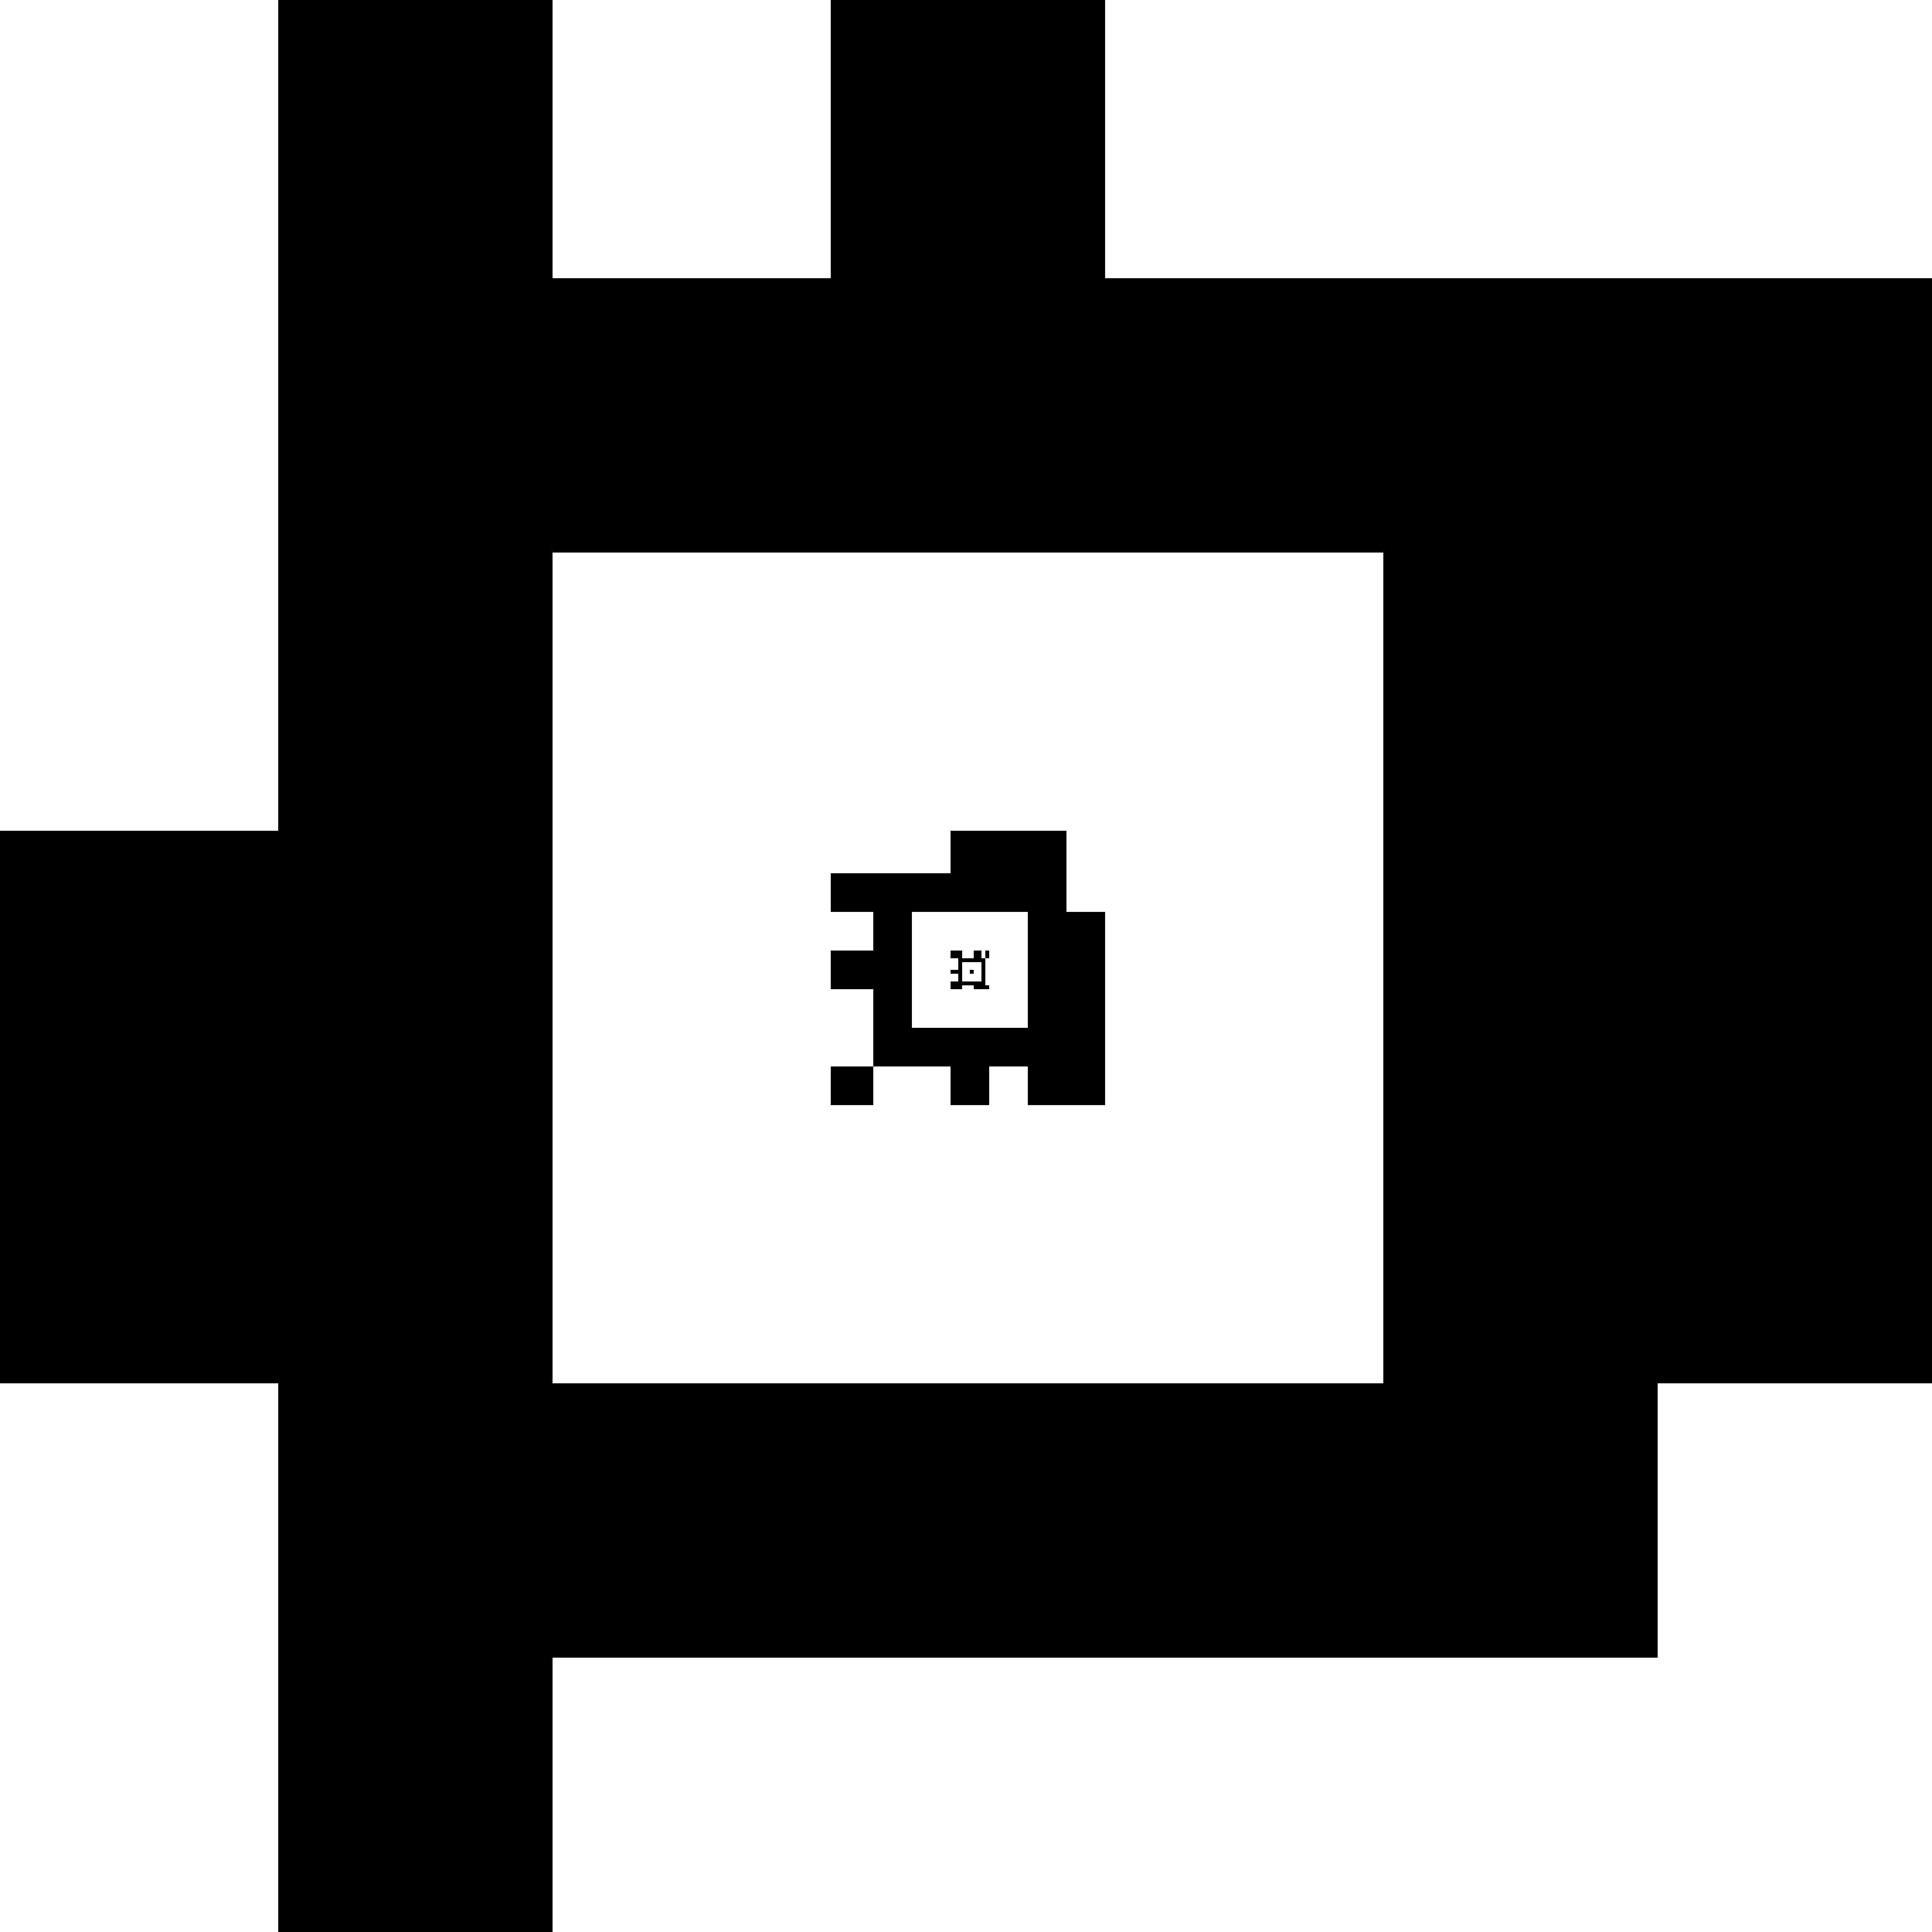
\includegraphics[width=\textwidth]{images/tagCustom24h10_00002_00001_00000}
        \caption{April Tag 24h10}
        \label{figure:apriltag24h10_example}
    \end{subfigure}
    \begin{subfigure}[b]{0.2\linewidth}
        
\includegraphics[width=\textwidth]{images/tagCustom48h12_00002_00001_00000}
        \caption{April Tag 48h12}
        \label{figure:apriltag48h12}
    \end{subfigure}

    \begin{subfigure}[b]{0.2\linewidth}
        
\includegraphics[width=\textwidth]{images/whycon_example}
        \caption{WhyCon}
        \label{figure:whycon}
    \end{subfigure}
    \begin{subfigure}[b]{0.2\linewidth}
        
\includegraphics[width=\textwidth]{images/tag_36h11_borderless}
        \caption{April Tag 36h11}
        \label{figure:apriltag36h11}
    \end{subfigure}
    \begin{subfigure}[b]{0.2\linewidth}
        
\includegraphics[width=\textwidth]{images/aruco_33}
        \caption{ArUco.}
        \label{figure:aruco33}
    \end{subfigure}
    \caption{Some examples of fiducial markers.}
    \label{figure:fiducial_markers}
\end{figure}

Fiducial markers are patterns whose pose (position + orientation) can be recognized
using only a monocular image and the camera parameters.
Figure \ref{figure:fiducial_markers} shows some common fiducial markers.
They can also provide a small bit of data as well, such as an idenfitier.
Often, fiducial markers are used to mark objects, so that the pose of the object itself
can be used to deduce the pose of the object it is attached to.
A common application of this is to allow a robot to locate and manipulate items.
Although the position of a fiducial marker is conceptually easy to determine from
a single monocular image, the orientation is subject to ambiguity
because of the inherently finite pixel resolution.
If the marker does not have sufficiently large pixel area, the sign of some of the
components of the orientation can flip unpredictably, meaning that the orientation
is not a reliable data point on which to make subsequent calculations.
See Section~\ref{section:fiducial_system_modifications}
for an analysis of this, and for some possible solutions.
